\section{Specification and design}
In this section we will be covering the specification and design of our program. The purpose of the specification is to provide a clear cut definition for what the program is supposed to do and how it is to be approached.

\subsection{Inputs and outputs}
In this section we will be specifying the inputs and outputs for our program.

\subsubsection{Input}\label{InputSpec}
As we mentioned in the requirements related to Input/Output, the native Excel file format \verb|.xlsx| is fairly complicated. We have decided that we will be using \verb|.csv| files instead. Excel has built-in functions for exporting and importing \verb|.csv| files, so this should still be fairly easy for the end user of the program to make use of.

The program should take a path to the input file as the first argument when invoking the program from the command line. This will in addition allow the program to be executed by drag and dropping a file onto the executable on Windows (and potentially other operating systems).

The output file should reuse the name of the input file with the word \textit{out} in-fixed between the end of the name and the file extension. Optionally the output file can be specified by providing the \verb|-o| flag followed by a file path when executing the program.

The input file we have been given as an example consists of seven columns and 13 rows of information. This is the information that would be available for a person manually fixing the schedule. Information like how many hours a team should have per day or week, or how many public holidays there are in a specific year. This means that the program should start from the eighth column and 14th row, and look at the rest of the sheet from that. The data that needs to be processed, is in the same format as seen in Table \ref{fig:Schedule no fix} which can be found on page \pageref{fig:Schedule no fix}. Additional information can be found in Section \ref{section:datadesc}.

\subsubsection{Output}
For the output file we are going to recreate the style that is used on \ref{fig:Schedule formated}. This can not be done perfectly since the end result is colour coded, and we are unable to encode colour information within a \verb|.csv| file. We are limited to specifying what information goes into each cell. Therefore we have to get a little creative. Each colour in the Excel file is going to get replaced by a character or symbol. Luckily there is not much text in the schedule so if we pick the right symbols it should be easy to find and replace the symbols with colour coding if the user really want to. The coding that we will be using is as follows:

\begin{itemize}
    \reqItem{Removed}{Green $\rightarrow$ RM}
    \reqItem{Added}{Blue $\rightarrow$ AD}
    \reqItem{SH-day}{Yellow $\rightarrow$ SH}
    \reqItem{Vacation}{Orange $\rightarrow$ VC}
\end{itemize}

The only one you can find in the schedule right now is RM, which shows up once. It should therefore be very easy to replace these if the user deems it necessary. 

%Now as for how we are going to write it to our output file. In our heads it might make more sense to calculate one month at a time, starting at the first one and then continuing chronologically. However, it makes much more sense computationally to do it row by row. This is because each line in the .csv file is a row in our schedule. We can make a single line at a time and write it to the .csv file, and then forget about it. However, working month to month is still possible, as the output will be a file that the program has full access to, meaning it can change every single line at any time if necessary.

One thing that we should keep track of though is all the special days. This being the SH-days, holidays, removed days and added days. We should definitely add this to the bottom of the schedule, as seen in the template. We need to show the information of these days as the user will have to mark these days with colours, and to check if any significant changes have been made.

The following figure (\ref{fig:Output_example}) shows an example of how the final work schedule should look:

\begin{figure}[ht!]
    \centering
    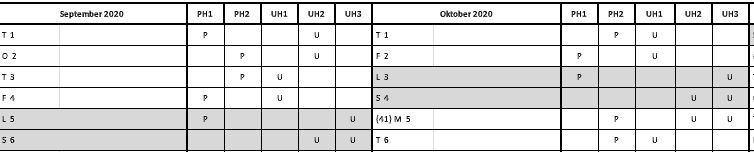
\includegraphics[width=\textwidth]{media/p1 schedule.JPG}
    \caption{The final work schedule example.}
    \label{fig:Output_example}
\end{figure}
 In the following chapter we will show how to read a \verb|.csv| file, which is also how we need to make the program write out the final file. Excel will then be able to show the final schedule by interpreting the \verb|.csv| file.

\subsubsection{Analysis of the input format}
\label{sec:input-analysis}
In this section we will be doing an in depth analysis of the input document format. The full document can be found through appendix \ref{appendix:local-agreements}.

The \verb|.csv| file format consist of multiple strings, separated by semicolons. Each string represents the value in the current column and each semi-colon represents the transition from one column to the next. Rows are separated by line breaks. Each row has the same total amount of semi-colons, this means that when a column is empty multiple semicolons may appear back-to-back.

A single day in the input timetable will be represented with the following line of data, in a \verb|.csv| file (note that the line is broken for the sake of readability, the listing represents one entire row):

\begin{lstlisting}[caption={Example row.}]
    9-1-2020;Tirsdag;;1;;;;P;6:00;18:00;11,50;;/
    ;;;0,00;;/;;;0,00;;U;18:00;6:00;11,50;
\end{lstlisting}

The first column contains the date, in this case \textit{"9-1-2020"}. The date is followed by the weekday in the proceeding column. In the next (third) column we can find the name of the SH-day, since the day used for this example is not an SH-day the column is left empty. For the next three columns the value is either omitted or \textit{"1"}. These columns are used to identify what kind of day it is, the first is always set and simply means that it is a day. The second column is used for identifying weekend days and the third for SH-days. The next column is always empty.

Then we reach a "P". This means that \primo team 1 has a shift this day. Then the hours come, from six to 18, and how many hours that is in paid work. Then two semicolons later, we meet a "/". This represents that the \primo team 2 does not have a shift this day. and therefore, there are no hours entered in the next two columns. Then the hours of the day is in the next column, and because there are no work hours, "0,00" is entered. The same is the case for the \ultimo team 1, that does not have a shift, and there therefore is a "/". The \ultimo team 2 however does have a shift, because there is a U, and then their hours. Then the next row of the Excel file will be on the next line. From now on we will not be showing the semicolon separated string, but instead the tables, as it is explained above how a table will be written as a semicolon separated file.

There is one more important information in the Excel file that we need our program to be able to read. That is the table at the top, that shows how many days, holidays, workdays and hours the different teams have with the current schedule.
 
\begin{figure}[ht!]
    \centering
    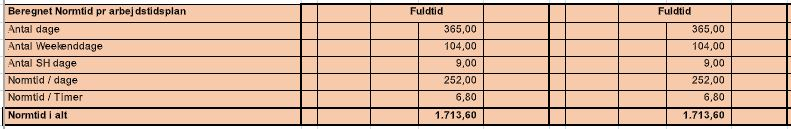
\includegraphics[width=\textwidth]{media/Table P2.JPG}
    \caption{Table of general information.}
    \label{fig:Table_information}
\end{figure}

We need to get the program to store the accumulated hours, as to know how many hours the teams should optimally have this year. The other information does not seem as important, as we will most likely gain the same values, when we store all the different days.


\subsubsection{In code representation of the input}
In this section we will be documenting some considerations we have made regarding the in-code representation of the input format.

As we went over in the section on input analysis (see \ref{sec:input-analysis}) the input source is a text file containing multiple rows each containing a series of information about the given time slot that the row represents. Since, we have many rows that all follow the same format the obvious solution is to make use of an array to store each row. It is however less obvious how to store the information contained within each of these rows.

The overall plan is to organize the contents of a row into a data structure. With that said we probably won't be using all the fields, since some information is slightly redundant. In addition, some representations used within the source data, would likely prove inconvenient to work with and as such we will be changing those to be more convenient.

The first field is the date of the given time slot. The original representation uses the following format \verb|day-month-year|. This should have its own data structure, with separate fields for month, day, and year.

The second field stores the name of the weekday. Instead of storing this as a string directly, we should convert it to a numeric representation with zero representing Monday and six representing Sunday. To represent this in code we will be using an enumeration type.

The third field is the name of the SH-day. This field is only needed for outputting text in the final schedule, as such it should simply be stored as a string.

As for the next three fields, they can be omitted since the other fields carry more than enough information to infer the value of these. For reference these fields state whether the time slot is on a day, a weekend day, or a SH-day.

For the remaining 20 fields there is a repeating pattern across four sections of five fields. The first of these five fields determines which team is working. The next two fields contain the start and end times for the shift respectively, the fourth contains how many work hours the shift is equivalent to. The last field is unused and will be omitted.

For the start and end times, we will be using a simple data structure with a field for hours and minutes. For the field containing the work hour count we will simply be using an integer for storing the work time in minutes (since minutes is the smallest unit used in this case). 
The time slots will be divided up into arrays based on the team it is associated with.

\begin{lstlisting}[caption={Example data structure.},language=C]
    typedef struct {
        Date date;
        Weekday day;
        const char* shName;
        Time startTime;
        Time endTime;
        int workHours;
    } Timeslot;
\end{lstlisting}

\subsection{Creating the work schedule}
In this section we will specify how our program will create the work schedule.

The program checks how many hours the current plan gives each team, and then calculates the difference between the planned hours and the hours agreed upon according to the union agreement. If the planned hours exceed the agreed upon hours by more than one shift, meaning 11.5 hours, the program should find the most optimal shift to remove. This means that the program should check if they are working on an SH-day, and remove that shift. If that is not possible it should then instead find a Saturday they work and remove that one. It should prioritize removing days that are particularly annoying to work on, such as days right before or after SH-days, or in periods of time when they have not had many days off. However, the program should also keep in mind, that we are going for constant production at \siemens, so we should not have a day with no shifts. We can allow a small team like Ultimo team 3 to close production alone, if it is more optimal to remove other shifts. The employees would most likely prefer this method over just choosing random days, since this method is more convenient.

On the other hand, if they are below the amount of hours needed, an extra shift should be added. The program needs to find a day that the team are not working and add a shift to that day. This day should also be carefully chosen. If a normal day is possible, it should be added there, but if that is not possible, then they should add it to a Saturday as far away from holidays as possible. Only if no such day exits should it place the shift on an SH-day.

\subsection{Program arguments}
In this section we will be specifying the syntax used for passing arguments to the program when invoking it through a command line shell.

When invoking the program from the command line, the user can pass along multiple arguments for the program. These options can be divided into two categories: main arguments and options. The overall syntax that is used when invoking the program can be seen in listing \ref{lst:OptionSyntax}.

\begin{lstlisting}[label={lst:OptionSyntax},caption={Syntax description for invocation of the program. Variable parts are marked as following: <variable>. Optional parts are marked as following: {[optional]}. As a shorthand for option, opt is used.},language=C]
<program> <main argument> [-<opt symbol> <opt value> ...]
\end{lstlisting}

The ordering of the arguments and options does not matter, but the program name must come before any arguments. While multiple options and main arguments are allowed, only the last main argument will be used. At least one main argument must be supplied. Options are of course optional.

An option consist of a symbol and a value. The symbol is preceded by a \verb|'-'| character. The symbol itself consists of a single ASCII character. The option value is a single string. How exactly a string is written depends on the shell used to invoke the program, but typically any characters up until the next whitespace character will be considered as part of the string. If whitespace is needed as part of the string the entire string should be enclosed between two '\verb|"|' (double-quote) characters.  Similarly to main arguments only the last of any duplicate options will be used --- options are considered duplicates if their symbols match.

Our program accepts the following option symbols: \verb|-o|, which as mentioned in section \ref{InputSpec} (input specification) can be used to specify the output file path, where the resulting schedule will be saved; \verb|-s,-l,-f,-S,-F| which are used to adjust weighting parameters, see section \ref{WeightingConfiguration} for more info; \verb|-c|, which is used to supply a file containing a list of criteria, see section \ref{CriteriaSpec}; and lastly \verb|-m|, which can be used to set the output mode (TODO insert reference once this has been documented).


\subsection{Criteria}\label{CriteriaSpec}
In this section we will specify the criteria option, and how the program will take the input from the user.

We want to take input from the user, regarding placement of some shifts. Say, the initial schedule gets rejected, you cannot use the program as it is again, since it will just output the same schedule. This can be prevented with the criteria option, where we want to take an input from the user, in a \verb|.csv| file where they specify: 
\begin{enumerate}
    \item The date that needs handling.
    \item If the team should work or not.
    \item What team needs this handling.
\end{enumerate}  

The information passed to the program should be made in the format shown on Listing \ref{lst:criteria_format}.
\begin{lstlisting}[caption={Format of Criteria}, label={lst:criteria_format}]
    DATE;X;TEAM
    DATE;X;TEAM
\end{lstlisting}
'\verb|DATE|' specifies the date in question. The date is formatted according to the following pattern: \verb|DD-MM-YYYY|. '\verb|X|' specifies if the team should work or not, which is determined with a '\verb|Y|' or an '\verb|N|' (Yes/No). '\verb|TEAM|' specifies which team is in question. The teams can be specified as follows:
\begin{itemize}
    \reqItem{PrimoOne}{\primo Team One}
    \reqItem{PrimoTwo}{\primo Team Two}
    \reqItem{UltimoOne}{\ultimo Team One}
    \reqItem{UltimoTwo}{\ultimo Team Two}
\end{itemize}
Each criteria should be put on its own line, and each specification should be separated with a semicolon, since we are working with a "Semicolon Separated Value" file-format (\verb|.csv|). On Listing \ref{lst:criteria_example} is an example of how a few lines could look like.
\begin{lstlisting}[caption={Example of criteria file}, label={lst:criteria_example}]
    21-12-2020;Y;PrimoOne
    19-1-2021;N;PrimoTwo
    20-4-2021;Y;UltimoOne
\end{lstlisting}

